\subsection{Speed Estimator}
\label{sec:speed}
Our system provides an estimation on the speed of each tracked vehicle, rising a visual alarm when the speed limits are exceeded. Other works on this field make use of the optical flow in order to make motion estimations, but this approach requires the conversion of pixels/frame to distance/time. Even though it is a feasible task, prior knowledge of pixels/distance ratio in the sequence is mandatory. Moreover, perspective generates a progressive distortion in this ratio along the regions of the image, which can be mitigated by the use of homography techniques. The need for a controlled test with a vehicle for calibration stands as a major drawback.\\ 

\noindent To avoid the above-mentioned problems we came up with a more straightforward approach based on a single estimation per track, reference points in the view field, and a known distance. This method does not need much calibration to achieve good results, and it requires fewer resources making its implementation simpler. We set 2 reference lines as seen in Fig. \ref{fig:layout} in the road and we compute the frame difference between the vehicle crossing the first marker and reaching the second one. Knowing the frame rate of the video and the distance between markers, speed is calculated by a simple equation. \\

\noindent This method relies on the assumption that the tracked detection is precise and the bounding box is considered the vehicle itself. This avoids the use of the detection's centroid, which introduces greater distortion in the relative distance to the marker line than a border does. It is most desirable that the vanishing point lies out of frame for the perspective to be less distorting. This assumption approximates the real case scenario quite well provided that the distance between markers is as big as possible. The further away the markers are with respect to each other, the less influence a distance error will have on the estimated speed.

\begin{figure}[t]
\centering
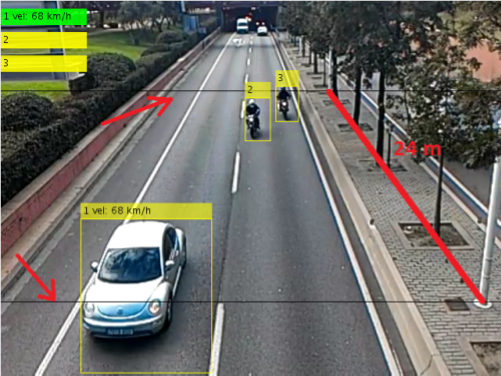
\includegraphics[width=0.9\linewidth]{figures/system}
\caption{System speed estimation layout with markers and distance pointed in red.}
\label{fig:layout}
\end{figure}

  